\subsection{Microsof Azure Formularerkennung}

In der Microsoft Produktfamilie der Azure Cognitive Services werden zahlreiche KI unterstützte Dienste, die zur Verbesserung 
und Automatisierung von Unternehemnssoftware dienen, bereitgestellt. Folgende Dienste für Text- und Bildanalyse stehen zur Verfügung:

\begin{enumerate}
    \item Form Recognizer
    \item Text Analytics
    \item Computer Vision
    \item Custom Vision
\end{enumerate}

Die Datenextraktion der firmeninternen Rechnungen erfolgt in dieser Arbeit mittels Form Recognizer bzw. Formularerkennung.
Der von Microsoft bereitgestellte Form Recognizer ist speziell auf das Extrahieren von einfachen Daten, wie Rechnungsdaten, 
Rechnungsnummern oder Anschriften der beteiligten Firmen ausgelegt. Aber auch komplexere Dokumentstrukturen, wie Tabellen können entnommen 
werden. 

Alle anderen erwähnten Dienste der Cognitive Services wie Computer Vision verfügen über die gleiche Grundfunktionalität, unterscheiden 
sich jedoch in Qualität, Spezifikation und im Ergebnis. Zum Beispiel ist der Dienst Custom Vision in der Lage zur reinen Textextraktion mithilfe von OCR,
Bilderkennung und Bewegungsanalysen, während der Form Recognizer darauf spezialisiert ist nur gewünschte, meist firmeninterne, Daten aus einem Formular zu entnehmen.

Für die Nutzung des Form Recognizer Dienstes, wird folgendes vorausgesetzt:
\begin{enumerate}
    \item Ressourcengruppe
    \item Formularerkennung
    \item Azure Speicherkonto
\end{enumerate}

\subsubsection{Ressourcengruppe}
Um die Formularerkennung nutzen zu können, ist die Erstellung einer Ressourcengruppen notwendig. Erstellt wird jene im Microsoft Azure Portal unter dem Menüpunkt "Ressourcengruppe erstellen".

\begin{figure}[h]
    \centering
    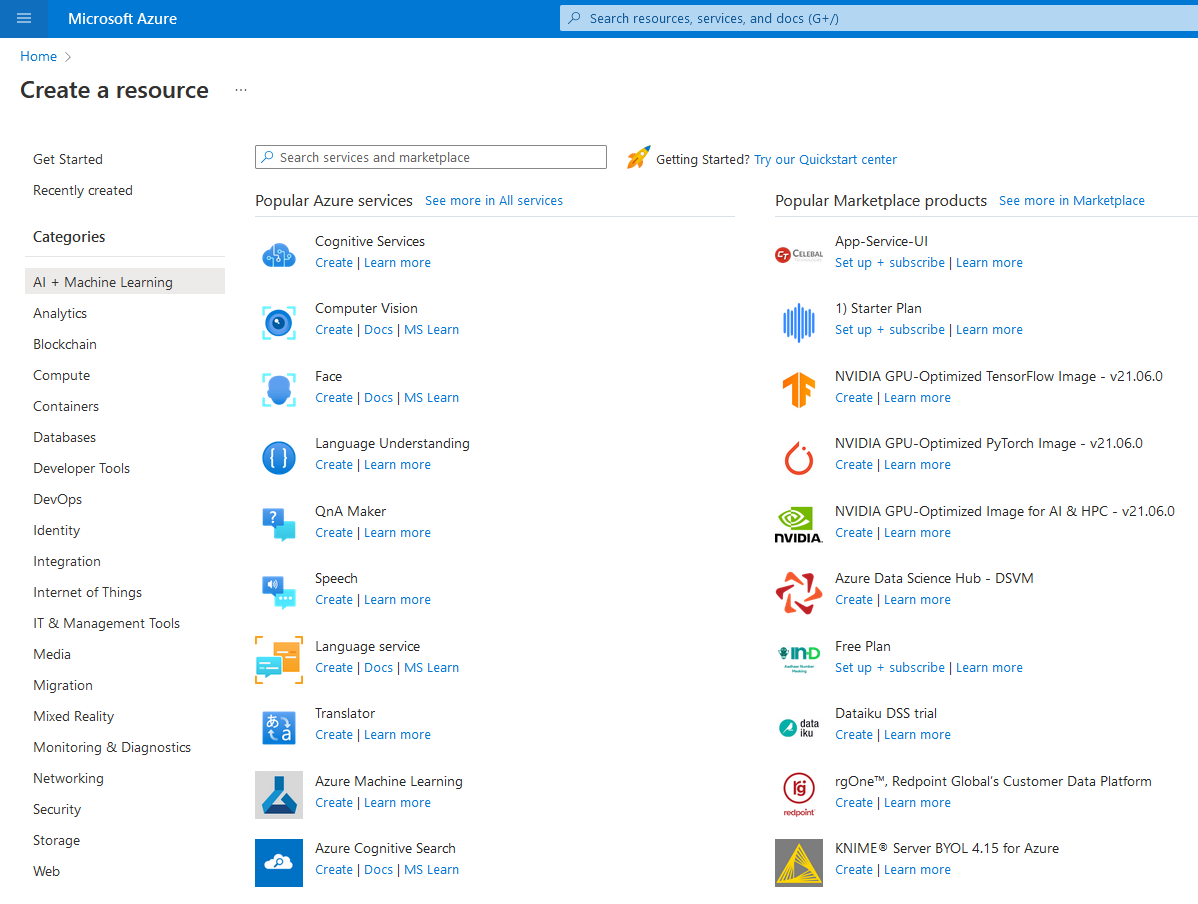
\includegraphics[scale=0.4]{sections/cloud-computing/images/ressourcengruppe.png}
    \caption{Ressourcengruppe erstellen}
    \label{fig:kimldl-comparison}
\end{figure}

\newpage In der folgenden Abbildung ist zu sehen, dass die Ressourcengruppe "CognitiveServices" genannt und die Serverregion auf
"(Europe) Germany West Central" gesetzt wurde. Die Wahl der Serverregion ist insofern relevant, da je nach Region die Verarbeitung der 
Daten unterschiedlich ist und somit auch die Datenschutzbestimmungen variieren.

\begin{figure}[h]
    \centering
    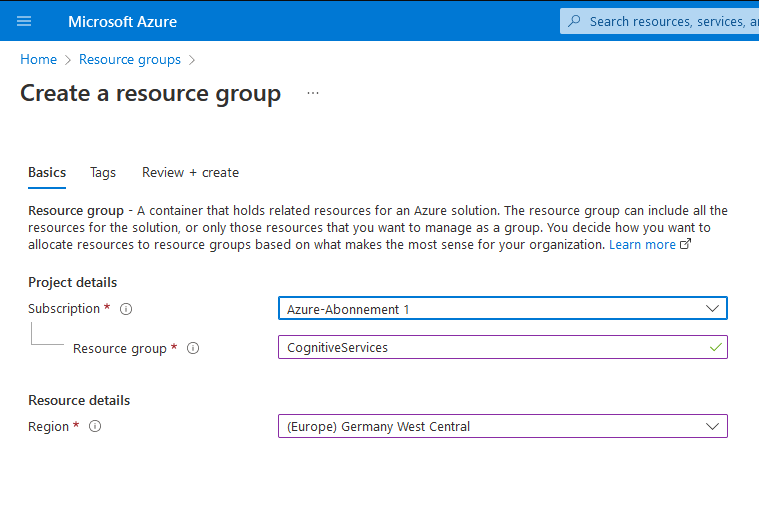
\includegraphics[scale=0.6]{sections/cloud-computing/images/ressourcengruppe-erstellen.png}
    \caption{Ressourcengruppe Details}
    \label{fig:formrecognizer-ressourcegroup}
\end{figure}

\subsection{Formularerkennung}
Im nächsten Schritt wird der eigentliche Cloud-Dienst erstellt. Gleich wie die Ressourcengruppe, ist die Formularerkennungsressource ebenfalls über 
den Menüpunkt "Ressource erstellen" hinzuzufügen.

Wie der nachstehenden Abbildung entnommen werden kann, wird der Cloud-Dienst der Formularerkennung der zuvor erstellten Ressourcengruppe "CognitiveServices"
zugewiesen. \ref{fig:formrecognizer-ressourcegroup}
Ebenfalls wurde die, auschließlich für den Umfang des Testzweckes, bestehende Preisebene "Standard S0" gewählt.


\begin{figure}[h]
    \centering
    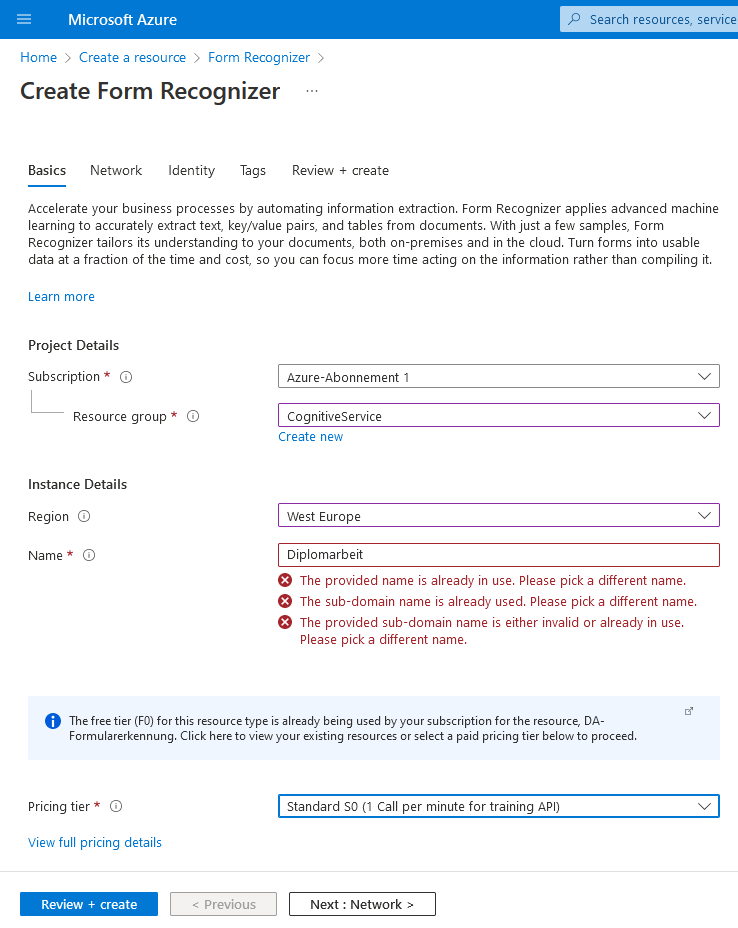
\includegraphics[scale=0.6]{sections/cloud-computing/images/formrecognizer.png}
    \caption{Ressourcengruppe erstellen}
    \label{fig:kimldl-comparison}
\end{figure}

\subsubsection{Azure Speicherkonto}\label{sec:azure-blob}
Um das Formularerkennungs-Modell später trainieren zu können, werden Trainingsdaten, bzw. Rechnungen im PDF-Format benötigt.
Diese werden in einem dafür erstellten Azure Blob-Speicherkonto festgehalten.

\textbf{Kurzer Exkurs; Blob}
bzw. \textbf{Binary large object} ist eine große Datei, meist Bild- oder Audiodatei, die wegen
ihrer besonderen Größe speziell verarbeitet und gespeichert werden muss. Wie der Name bereits verrät 
werden große Mengen an unstruktierten binären Daten in einer Blob-Datei gespeichert.

Um ein Speicherkonto zu erstellen müssen die Menüpunkte "Ressource erstellen" und "Speicherkonto" ausgewählt werden. Ebenso wie
bei der Formularerkennungsressource muss die überstehende Ressource "CognitiveServices" verknüpft werden.

\begin{figure}[h]
    \centering
    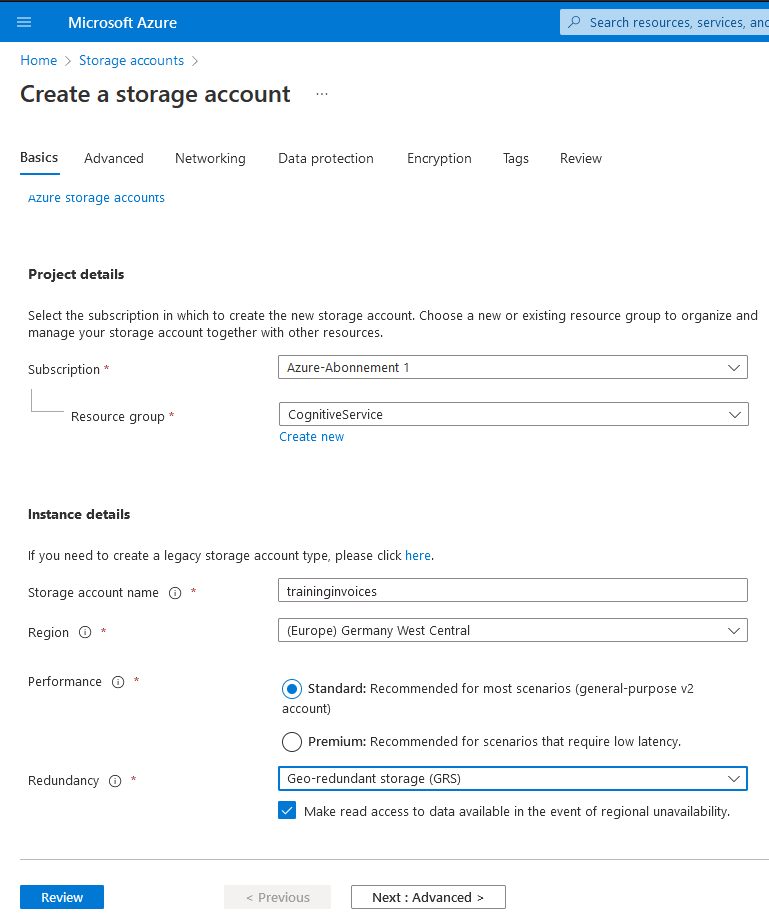
\includegraphics[scale=0.6]{sections/cloud-computing/images/azure-speicherkonto.PNG}
    \caption{Ressourcengruppe erstellen}
    \label{fig:ressourcen-erstellen}
\end{figure}

Anschließend können alle zuvor erstellten Ressourcen im Menüpunkt "Alle Ressourcen" eingesehen werden, wie in Abbildung \ref{fig:ressourcen-überblick} zu sehen ist

\begin{figure}[h]
    \centering
    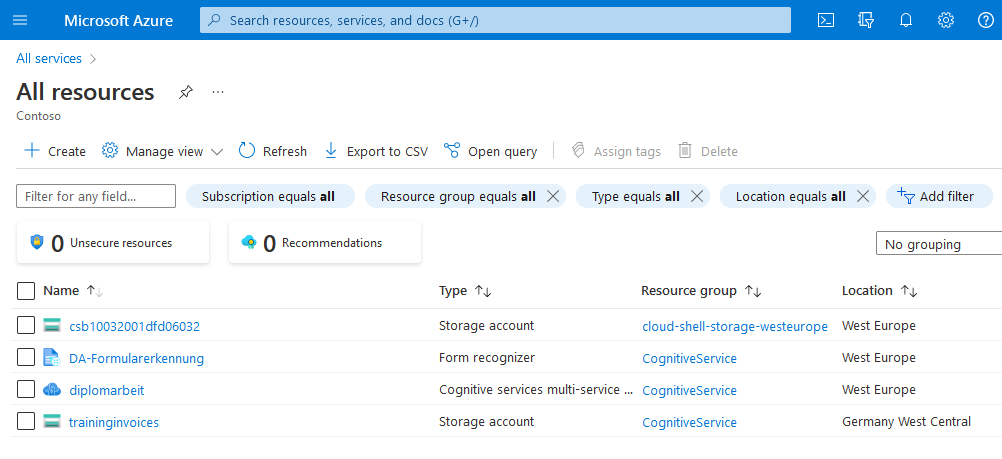
\includegraphics[scale=0.6]{sections/cloud-computing/images/alle-ressourcen.PNG}
    \caption{Ressourcen im Überblick}
    \label{fig:ressourcen-überblick}
\end{figure}

Im nächsten Schritt wird das Modell erstellt und trainiert, um den Dienst Formularerkennung zu nutzen. Zunächst wird das UI zur Erstellung 
des Modells benötigt. Mit dem nachfolgenden Link ist diese zu erreichen: 

\begin{center}\url{https://fott-2-1.azurewebsites.net/}\end{center}

Um ein eigenes Modell zu erstellen muss, wie in der folgenden Abbildung zu sehen ist, der dritte Punkt "Use Custom to train a model with labels and get key value pairs"
ausgewählt werden

\begin{figure}[h]
    \centering
    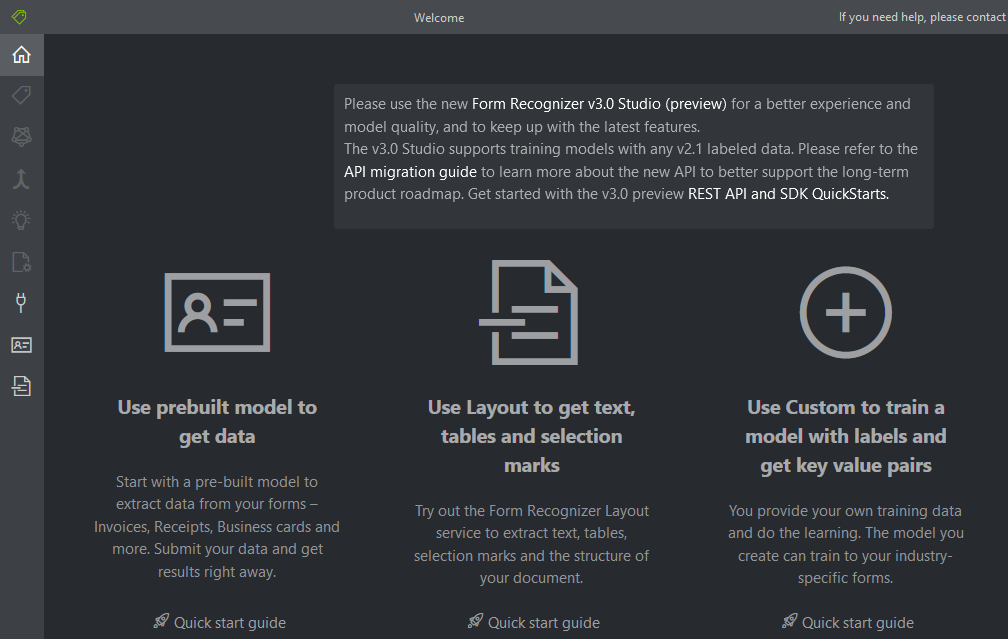
\includegraphics[scale=0.4]{sections/cloud-computing/images/formrecognizer-UI.PNG}
    \caption{Startseite formrecognizer UI}
    \label{fig:formrecognizer-UI}
\end{figure}

Als nächstes muss eine Verbindung zwischen dem zuvor erstellten Azure Blob Speicherkonto, und dem Projekt erzeugt werden. Erforderliche Eingaben sind Verbingsname
und SAS (Shared Access Signature) URI. Diese SAS URI muss zuvor im Azure Portal in der Übersicht des Azure Blob Speicherkonto generiert werden.

\begin{figure}[h]
    \centering
    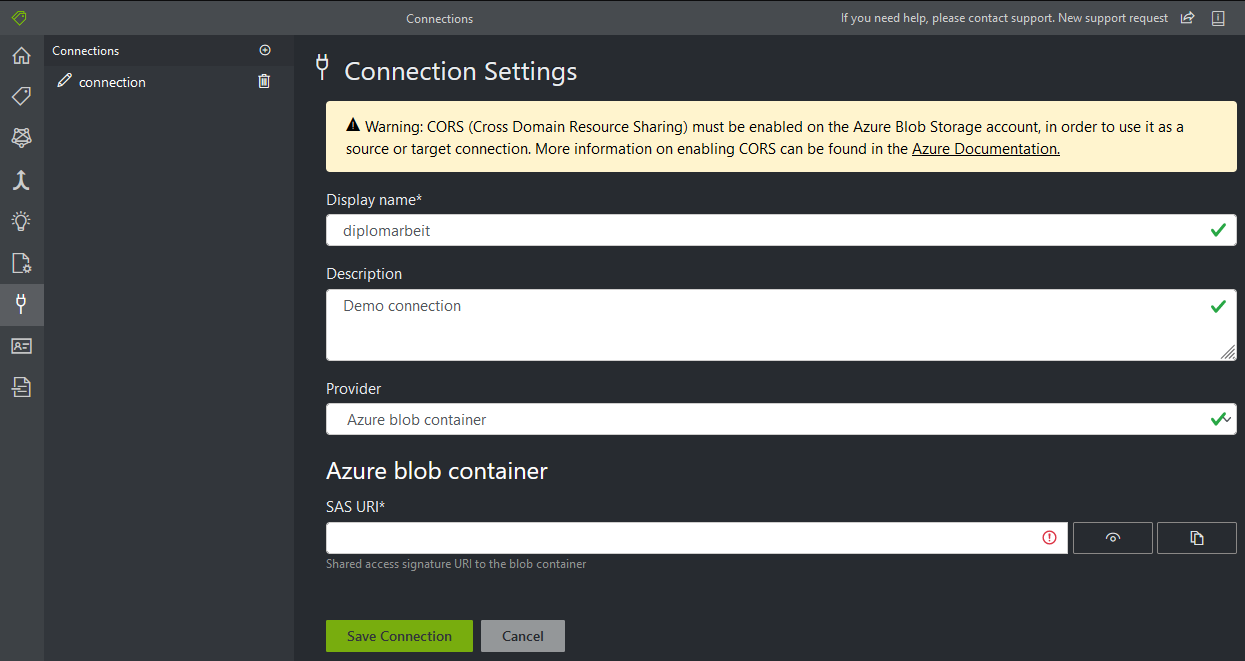
\includegraphics[scale=0.5]{sections/cloud-computing/images/formrecognizer-blob-connection.PNG}
    \caption{Erstellen der Verbindung}
    \label{fig:formrecognizer-blob-connection}
\end{figure}

Im nächsten Schritt muss ein sogenannter Security token erstellt werden. Dieser kann im Azure Portal in der Formrecognizerressource erstellt werden.
Als Name für den Security token wurde "DA-Formrecognizer Token" gewählt. Siehe nachstehende Abbildung \ref{fig:formrecognizer-security-token}.

\begin{figure}[h]
    \centering
    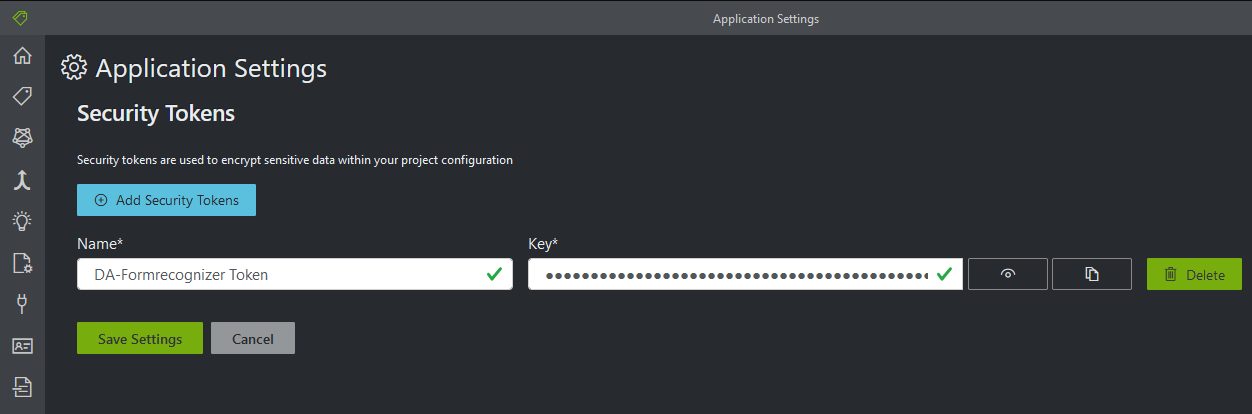
\includegraphics[scale=0.5]{sections/cloud-computing/images/formrecognizer-security-token.PNG}
    \caption{Erstellen der Verbindung}
    \label{fig:formrecognizer-security-token}
\end{figure}

Als finalen Schritt muss jetzt das eigentliche Projekt erstellt werden. Dazu muss im Hauptmenü des Formrecognizer-UI der Punkt "Neues Projekt"
gewählt werden. Um ein Projekt zu erstellen, sind folgende Eingaben essentiell: 

\begin{enumerate}
    \item Security token
    \item Source connection
    \item Formrecognizer URL
    \item API key
\end{enumerate}

Den zuvor erstellten Security token und die connection im Drop-down Menü, der jeweilig zugöhiregn Zeile, auswählen und Formrecognizer URL und API key eingeben.
Die beiden Eingaben "Formrecognizer URL" und "API key", können im Azure Portal in der Formrecognizerressource gefunden werden. Somit ist 
Erstellung und Konfiguration der Formrecognizerressource abgeschlossen und es kann mit dem Trainieren des Modells begonnen werden.

\begin{figure}[h]
    \centering
    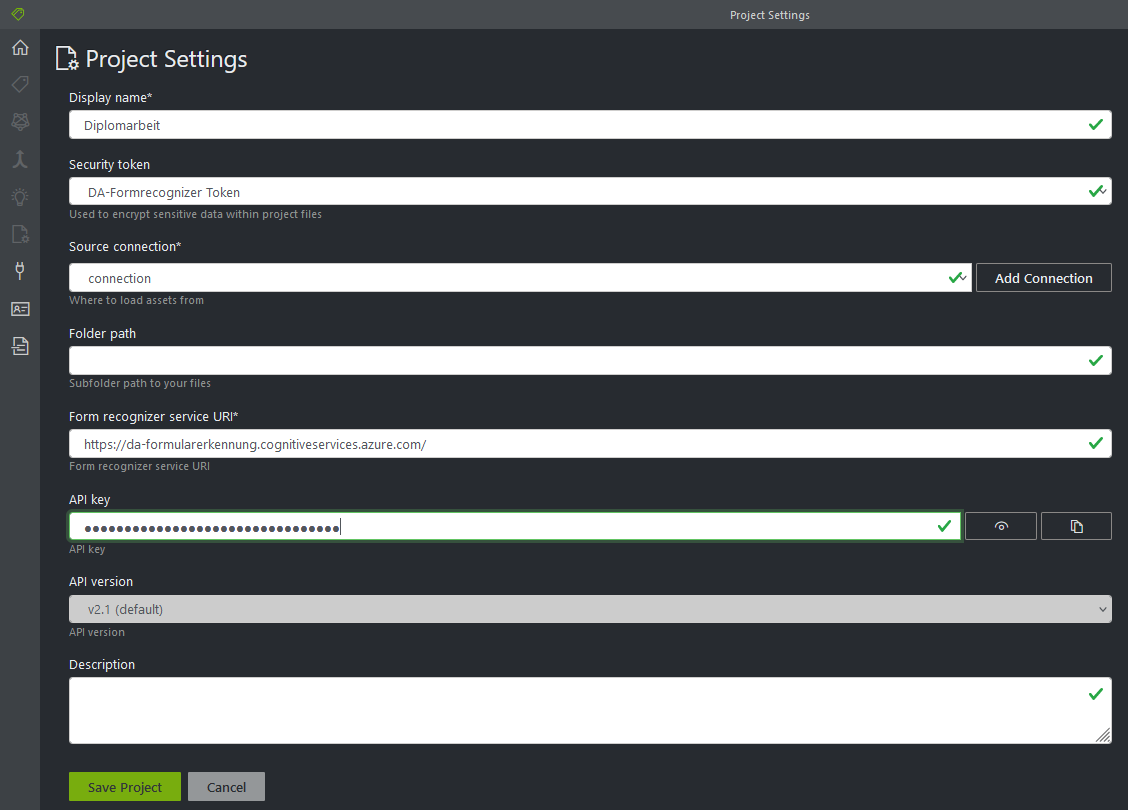
\includegraphics[scale=0.5]{sections/cloud-computing/images/formrecognizer-new-project.PNG}
    \caption{Erstellen der Verbindung}
    \label{fig:formrecognizer-security-token}
\end{figure}

\subsubsection{Trainieren des Modells}

Mit den vorherigen Schritten wurde die Konfiguration der Formularerkennungsressource abgeschlossen. In den folgenden Schritten wird das 
Anlernen der firmeninternen Rechnungen und die darausfolgende Analyse beschrieben.
Durch die Auzure Formularerkennung werden dem Benutzer zwei Möglichkeiten, zum Trainieren des Modells, zur Verfügung gestellt:

\begin{enumerate}
    \item das Benutzen von vordefinierten Dokumenten 
    \item benutzerdefinierte Dokumente
\end{enumerate}

Entsprechend der im vorhinein festgelegten Rahmenbediengungen dieser Arbeit, wurden benutzerdefinierte Dokumente, bzw. Rechnungen benutzt.
Bei benutzerdefinierten Dokumenten ist der Benutzer im Stande, das Modell auf den Aufbau und Inhalt firmenspezifischer Rechnungen zu trainieren.
Das Modell erlernt hierbei, wie Felder bzw. Rechnungselemnte zusammenhängen, und versucht Muster in den verschiedenen Trainingsdaten zu erkennen, und später
bei der Analyse anzuwenden. 

Es wird von Microsoft empfohlen, für jede Dokumentenkollektion fünf oder mehr Dokumente hochzuladen. Um dieser Empfehlung nachzukommen, wurden zehn Rechnungskollektionen von Eingangsrechnungen, mit jeweils vier bis sechs Rechnungen zum Trainieren und weitere zwei bis vier zum Testen in den Azure Blob Speicher geladen. Um das Modell trainieren zu können, wurde in den vorherigen Schritten ein Azure Blob Speicherkonto erstellt (\ref{sec:azure-blob}). Die in dem Blob-Speicher enthaltenen Rechnungen werden automatisch in die Cloud geladen und in dem Formrecognizer UI angezeigt. Die OCR-Software erkennt nach kurzer Wartezeit alle Zeichen und kennzeichnet diese. Weiters müssen anschließend, die von der OCR-Software erkennten Zeichen markiert und den gewünchsten Feldern zugewiesen werden. Diese Zuweisung ist essentiell, um dem Modell eine gewisse Dokumentstruktur zu erlernen. Deshalb wurden das Austellungsdatum dem Tag "Invoice Date" und der Gesamtbetrag der Rechnung "TotalValue" zugewiesen.
Siehe Abbildung \ref{fig:formrecognizer-invoice-tagging}

\begin{figure}[h]
    \centering
    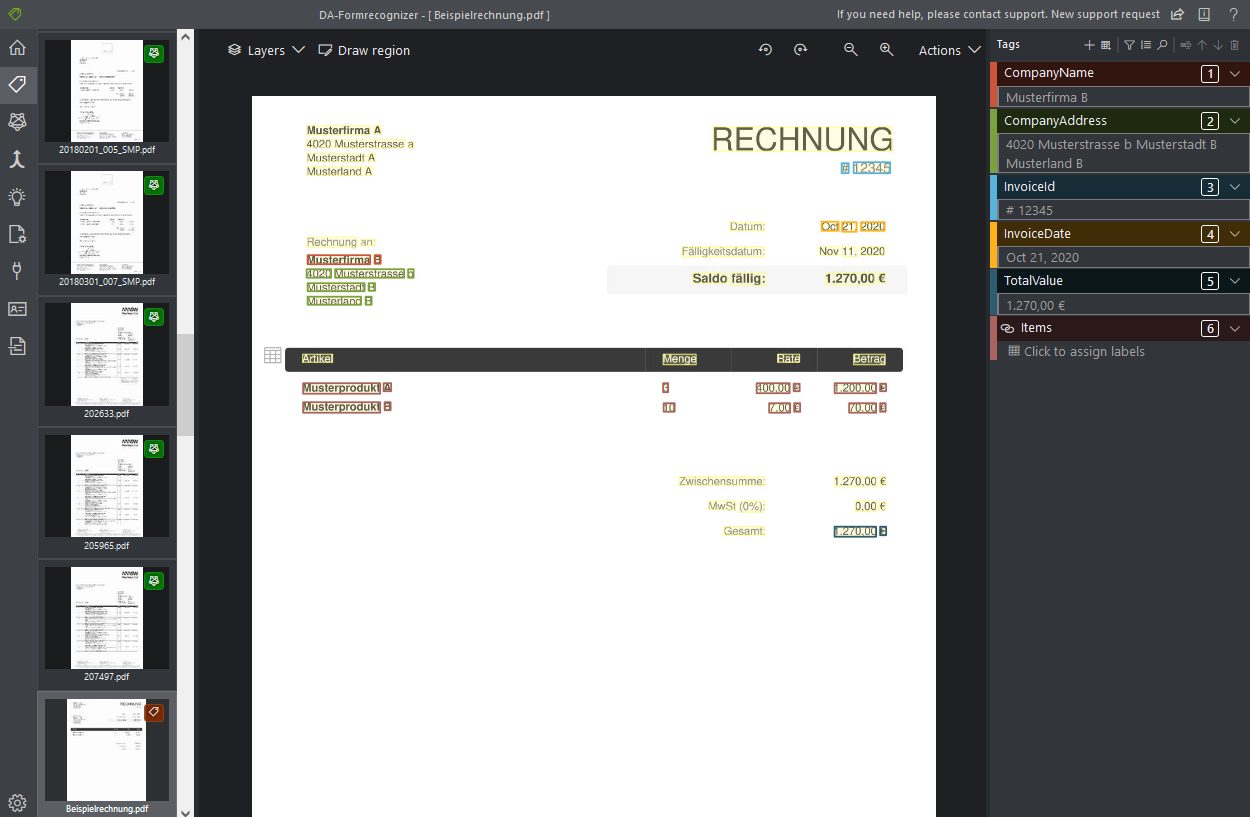
\includegraphics[scale=0.4]{sections/cloud-computing/images/formrecognizer-invoice-tagging.PNG}
    \caption{Übersicht}
    \label{fig:formrecognizer-invoice-tagging}
\end{figure}

Um tabellarische Daten markieren zu können, wird ein spezieller Tag-Typ benötigt, der sogenannte "table tag". Wie in der folgenden Abbildung 
\ref{fig:formrecognizer-invoice-tagging-items} zu sehen ist, können mehrere Zeilen abermals mit verschiedenen eigenen Tags versehen werden.

\begin{figure}[h]
    \centering
    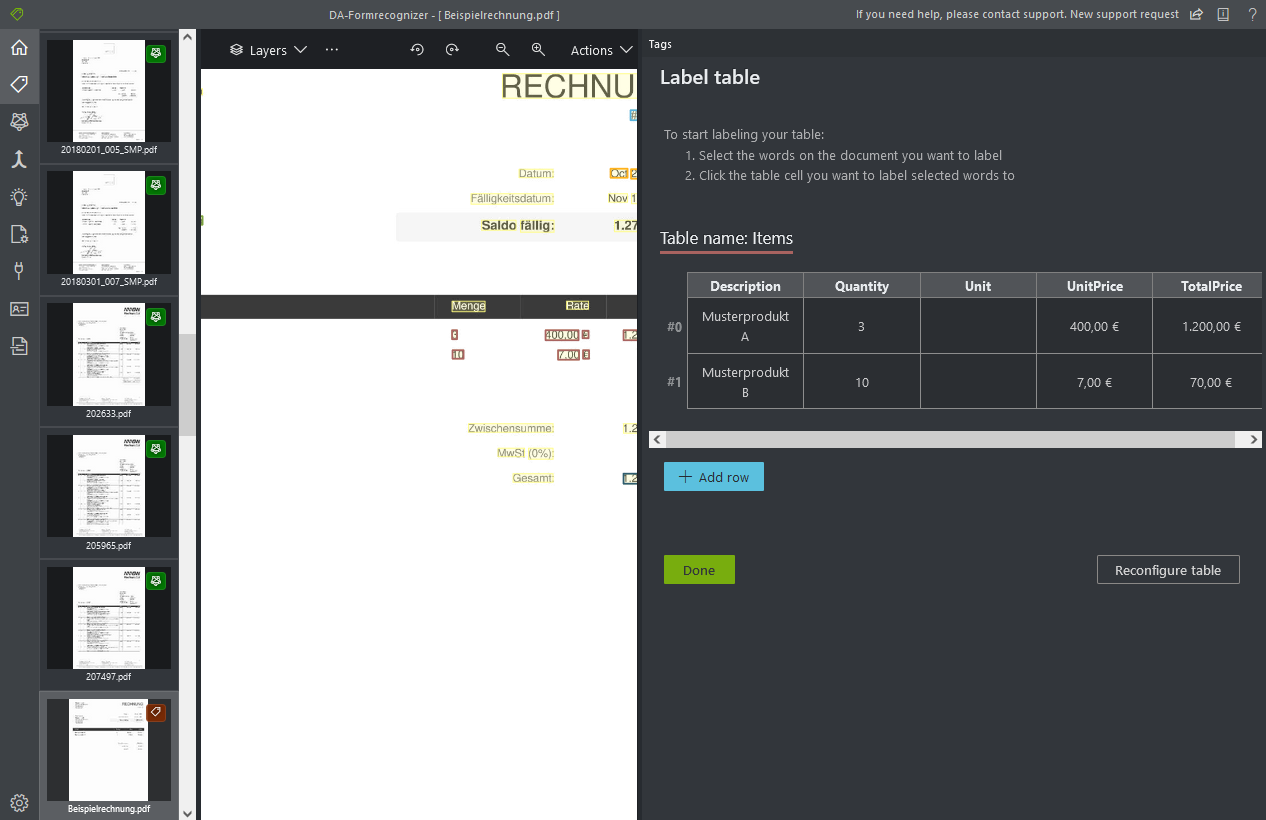
\includegraphics[scale=0.4]{sections/cloud-computing/images/formrecognizer-invoice-tagging-items.PNG}
    \caption{Tagging der Rechnungsfelder}
    \label{fig:formrecognizer-invoice-tagging-items}
\end{figure}

Wenn alle Dokumente erfolgreich markiert wurden, kann das Modell im Menüpunkt "Train" trainiert werden. Somit eignet sich die Formularerkennung, anhand der 
verfügbaren Daten, die Dokumentstruktur jeder einzelnen Rechnungskollektion an. Das Ergebnis wird in der folgenden Abbildung dargestellt.

\begin{figure}[h]
    \centering
    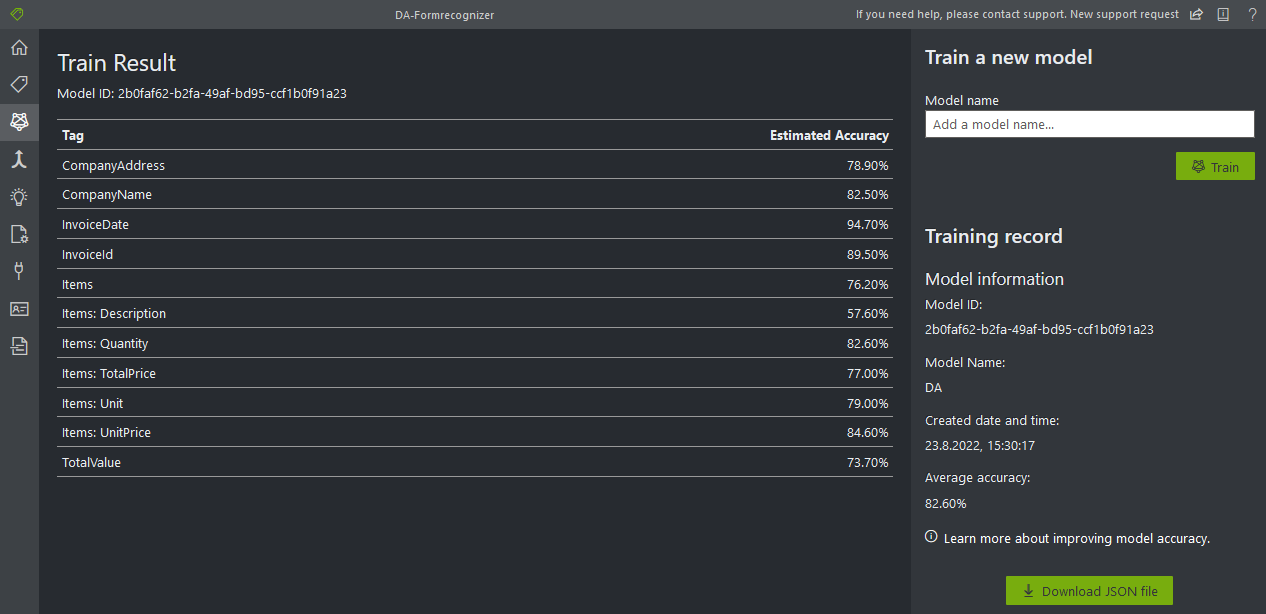
\includegraphics[scale=0.4]{sections/cloud-computing/images/formrecognizer-model-overview.PNG}
    \caption{Übersicht des Modells}
    \label{fig:formrecognizer-invoice-tagging-items}
\end{figure}

\subsubsection{Zusammenfassung und Ergebnis der Formularerkennung}